%% This is an example first chapter.  You should put chapter/appendix that you
%% write into a separate file, and add a line \include{yourfilename} to
%% main.tex, where `yourfilename.tex' is the name of the chapter/appendix file.
%% You can process specific files by typing their names in at the 
%% \files=
%% prompt when you run the file main.tex through LaTeX.

\singlespacing{

\chapter{Future Work}\label{chap:futureWork}

Future work revolves around hierarchical extensions of the current CAD/simulation model, experiments in computational design optimization, and development of a video game around digital materials.

\section{Hierarchical Simulation}

\begin{figure}
  \includegraphics[width=\textwidth]{FunctionsParts.png}
  \caption{Three functional primitives decomposed as assemblies of elements.  The geometrical layout of elements within a functional primitive establish its mechanical and electronic properties.  Two sketches of a 1DOF Bending Flexure have different mass, moment of inertia, conductivity, and bending stiffnesses (top, middle).  Parallel plate construction of a capacitor from conducting and insulating parts determines the functional primitive's global capacitance (bottom).}
  \label{fig:FunctionsParts}
\end{figure}

The hierarchical scaling of structure and function in our assembly system (Chapter \ref{chapter:HierarchicalDesign}) hints to a hierarchical framing of design and simulation in software.  The bulk of this thesis explores CAD/simulation at the function-level, especially the decomposition of functional parts into functional primitives.  Future work will explore design and simulation at other levels of hierarchy and translate behaviors of assemblies at one level into higher-level building blocks.\\

Current thoughts around the translation of \textit{assemblies of elements} to \textit{functional primitives} are depicted in Figures \ref{fig:FunctionsParts} and \ref{fig:HierarchicalSim}.  Mechanical parameters describing a functional primitive are calculated from static simulations of assemblies of elements.  Boundary conditions applied to elements at each face of an assembly induce steady-state deformations; 15 sets of boundary conditions apply forces from which $F = kx$ and $T = k\theta$ may be solved for all 15 stiffness constants.  Additionally, the inertia tensor and mass are computed directly from constituent material densities and geometry.  For example, differences in composition between the two 1DOF bending flexures depicted in Figure \ref{fig:FunctionsParts} are expressed as differences in stiffness constants, mass, and inertia at the functional primitive level of description (Figure \ref{fig:HierarchicalSim}).  In the case that mechanical deformations are not linear over a range of applied forces, a constant $k$ is calculated to best fit the data.  \\

Electronic properties may be determined as well.  Conductance between faces of a functional primitive are trivially calculated from assemblies of conducting and insulating elements.  Static capacitance and inductance are computed using steady-state solutions to Finite Difference Time Domain (FDTD) simulations; previous work in DMDesign used FTDT to calculate potential fields (Figure \ref{fig:designAssemblyGUIWide}E).\\

\begin{figure}
  \includegraphics[width=\textwidth]{HierarchicalSim.png}
  \caption{Schematic view of the translation of an assembly of elements into functional primitive parameters: 15 stiffness constants, mass, and moment of inertia tensor.  Blue boxes indicate ``attachment points'' for applied boundary conditions in multidimensional stiffness measurements.}
  \label{fig:HierarchicalSim}
\end{figure}

Modules and complexes exhibit high-level behaviors that are abstracted from the low-level physics of the system.  Simulation of modules and complexes may reflect this abstraction by modeling interactions with a discretized, kinematic CA ruleset (somewhat like the work of William Stevens with CBlocks3D \cite{Stevens2009b}).  At this time it is still unclear how to generate a module's governing ruleset from behaviors of assemblies of function-level parts.

\section{Declarative Design}

A long term goal of this work is to close the loop between CAD and simulation and move towards \textit{declarative design}.  In a declarative design workflow, users specify high-level goals and a constrained optimization process searches across parameter space for a solution.  The discretization of space and finite set of parts types at each level hierarchy within our assembly system sets it up nicely for constrained design optimization.\\

Once a method of translating assemblies of elements into functional primitives has been established (see discussion from previous section), we can perform topology optimization across assemblies of elements to discover new types of functional primitives (Figure \ref{fig:DeclarativeDesign}).  Fabrication limitations should be translated into geometric constraints to ensure that the outcomes of the optimization are reasonable.  Future work could also explore optimization of control strategies for actuated assemblies, similar to previous work by Sims \cite{Sims1994}.

\begin{figure}
  \includegraphics[width=\textwidth]{DeclarativeDesign.png}
  \caption{A 1DOF bending flexure is optimized in a topology optimization process.  Variations on initial user-generated design are evaluated in simulation.  This design/simulation loop is repeated until fabrication constraints and high-level goals are satisfied.}
  \label{fig:DeclarativeDesign}
\end{figure}

\section{``Fab the Game''}

An offshoot of the work described in this thesis is a collaboration with \href{http://elinemedia.com/}{E-Line Media} on a game.  Tentatively called ``Fab the Game'', it explores an aspirational future where digital materials are used to construct nearly everything.  In the game, players construct assemblies from functional primitives in an open-ended sandbox environment and in more directed challenges.  We envision a large component of gameplay revolves around constructing robots, operating them, and using them to shape the surrounding environment.\\

The game will extend the physical simulation outlined in Chapter \ref{chap:functionSim} through realtime user interaction.  For example, actuators in the game can be mapped to the keyboard and other gaming controllers so players can operate their robots in realtime.  Complex robots may be driven by a combination of preprogrammed controls and user input.  Using these controls, players test the agility and speed of their robot in arena challenges, drawing inspiration from the competitions of \href{http://www.firstinspires.org/robotics/frc}{First Robotics}.\\

More advanced modes of gameplay borrow from the ideas discussed in the previous two sections.  Players dive into functional primitive definitions and alter their elemental composition to unlock new functional properties beyond those available by default.\\

Through this game, we hope to familiarize players with CAD and simulation tools, constraint-based machine design, controls, and design optimization.  We will also provide offramps to digital fabrication workflows so that designs may be realized IRL (``in real life'') by gamers/makers.  In order to ease the burden of building large assemblies of parts, we may introduce concepts in hierarchical and parametric design within the crafting interface.  We are curious to see what players are able to construct within the game and hope it might inform future research trajectories at CBA.\\

Concept art by Eli Gershenfeld explores the look and feel of the game as well as potential gameplay scenarios (Figures \ref{fig:elibendy} through \ref{fig:elibridgefull}).

\clearpage

\begin{figure}
  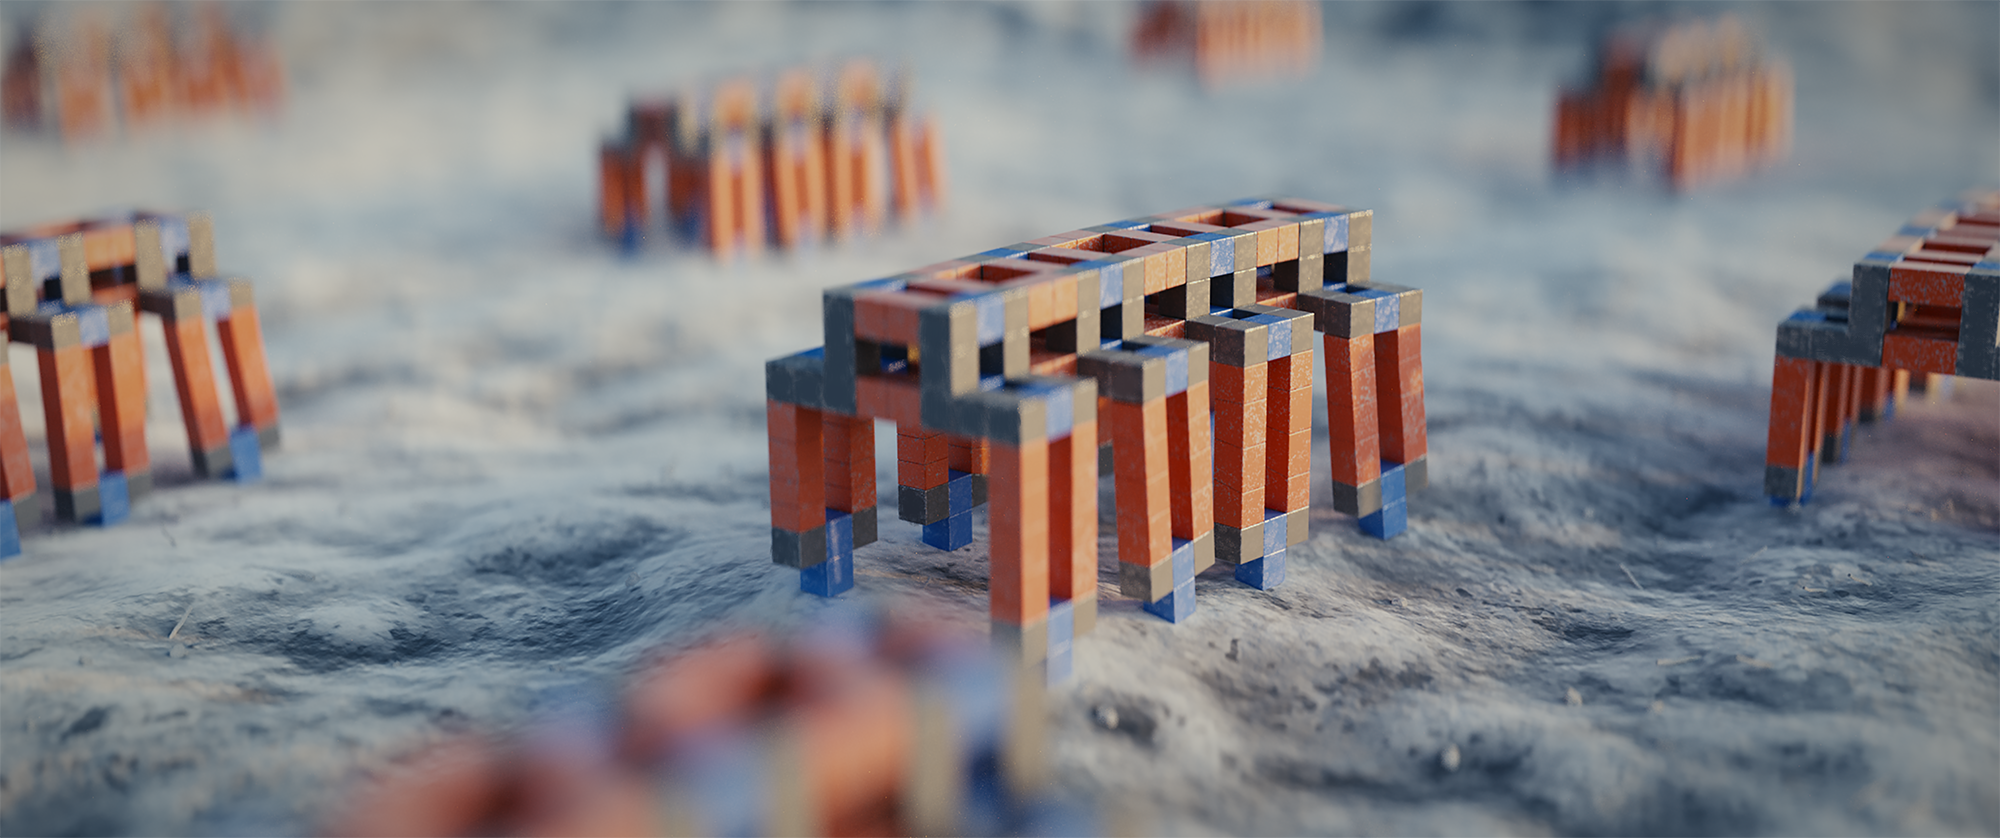
\includegraphics[width=\textwidth]{elibendy.png}
  \caption{A swarm of locomoting robots.  \textit{Image Credit: Eli Gershenfeld 2016}}
  \label{fig:elibendy}
\end{figure}

\begin{figure}
  \includegraphics[width=\textwidth]{eliassemblers.png}
  \caption{Assembler assembling an assembler.  \textit{Image Credit: Eli Gershenfeld 2016}}
  \label{fig:eliassemblers}
\end{figure}

\begin{figure}
  \includegraphics[width=\textwidth]{eliassembclose.png}
  \caption{Assembler ``factory'' feedstock.  \textit{Image Credit: Eli Gershenfeld 2016}}
  \label{fig:eliassembclose}
\end{figure}

\begin{figure}
  \includegraphics[width=\textwidth]{eliassembwide.png}
  \caption{Distributed ``factory'' automation. \textit{Image Credit: Eli Gershenfeld 2016}}
  \label{fig:eliassembwide}
\end{figure}

\begin{figure}
  \includegraphics[width=\textwidth]{elibridgeclose.png}
  \caption{``Living'' macro-scale structure.  \textit{Image Credit: Eli Gershenfeld 2016}}
  \label{fig:elibridgeclose}
\end{figure}

\begin{figure}
  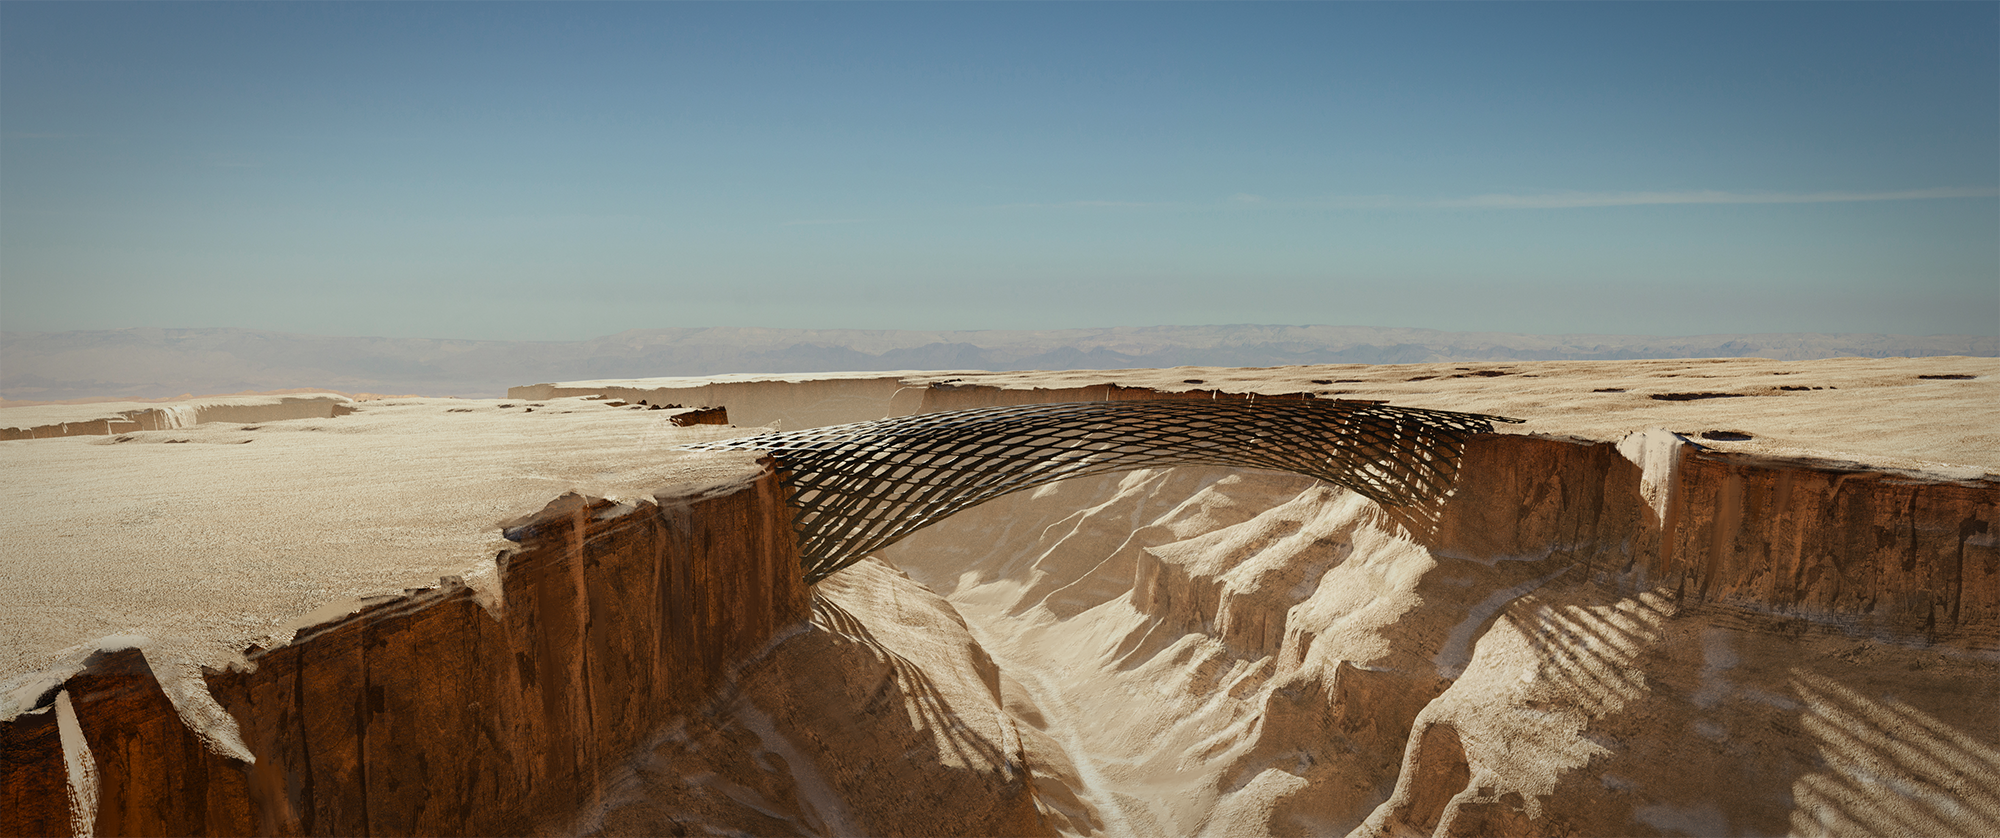
\includegraphics[width=\textwidth]{elibridgefull.png}
  \caption{Self-assembling bridge. \textit{Image Credit: Eli Gershenfeld 2016}}
  \label{fig:elibridgefull}
\end{figure}

